% Generated by tex/build_swebok_structure.py from tex/chapters/ch01/04_要求獲得.tex
\subsubsection{一般的な要求獲得技法}

要求獲得には多くの技法がある。技法は相手や目的によって使い分ける。

\par\smallskip\noindent\refstepcounter{table}\label{tab:ch01-07}\textbf{表 \thetable: 第01章 ソフトウェア要求 表07}\par\smallskip
\begin{tabularx}{0.97\linewidth}{@{}p{.25\linewidth}X@{}}
\toprule
技法 & 何に向いているか \\
\midrule
\term{面接} & 個別の経験、例外処理、暗黙知を聞き出す。 \\
\term{会議・討議} & 複数の関係者で認識を合わせる。 \\
\term{促進付きワークショップ} & 利害関係者を集め、短時間で合意形成や要求整理を行う。 \\
\term{質問票・市場調査} & 多数の人から傾向を集める。 \\
\term{観察} & 現場作業や実際の利用状況を確認する。 \\
\term{徒弟型学習} & ソフトウェア技術者が実際の作業を体験し、暗黙知を得る。 \\
\term{試作} & 画面や操作感を具体化し、利用者から反応を得る。 \\
\term{ユーザーストーリーマッピング} & 利用者の行動の流れに沿って機能を整理する。 \\
\term{文献・標準調査} & 法規制、標準、既存仕様に基づく要求を見つける。 \\
\bottomrule
\end{tabularx}

\begin{figure}[htbp]
\centering
\IfFileExists{swebok_structure/CH01.ソフトウェア要求(Software_Requirements)/1.2.要求獲得(Requirements_Elicitation)/1.2.2.一般的な要求獲得技法(Common_Requirements_Elicitation_Techniques)/assets/fig-ch01-06.png}{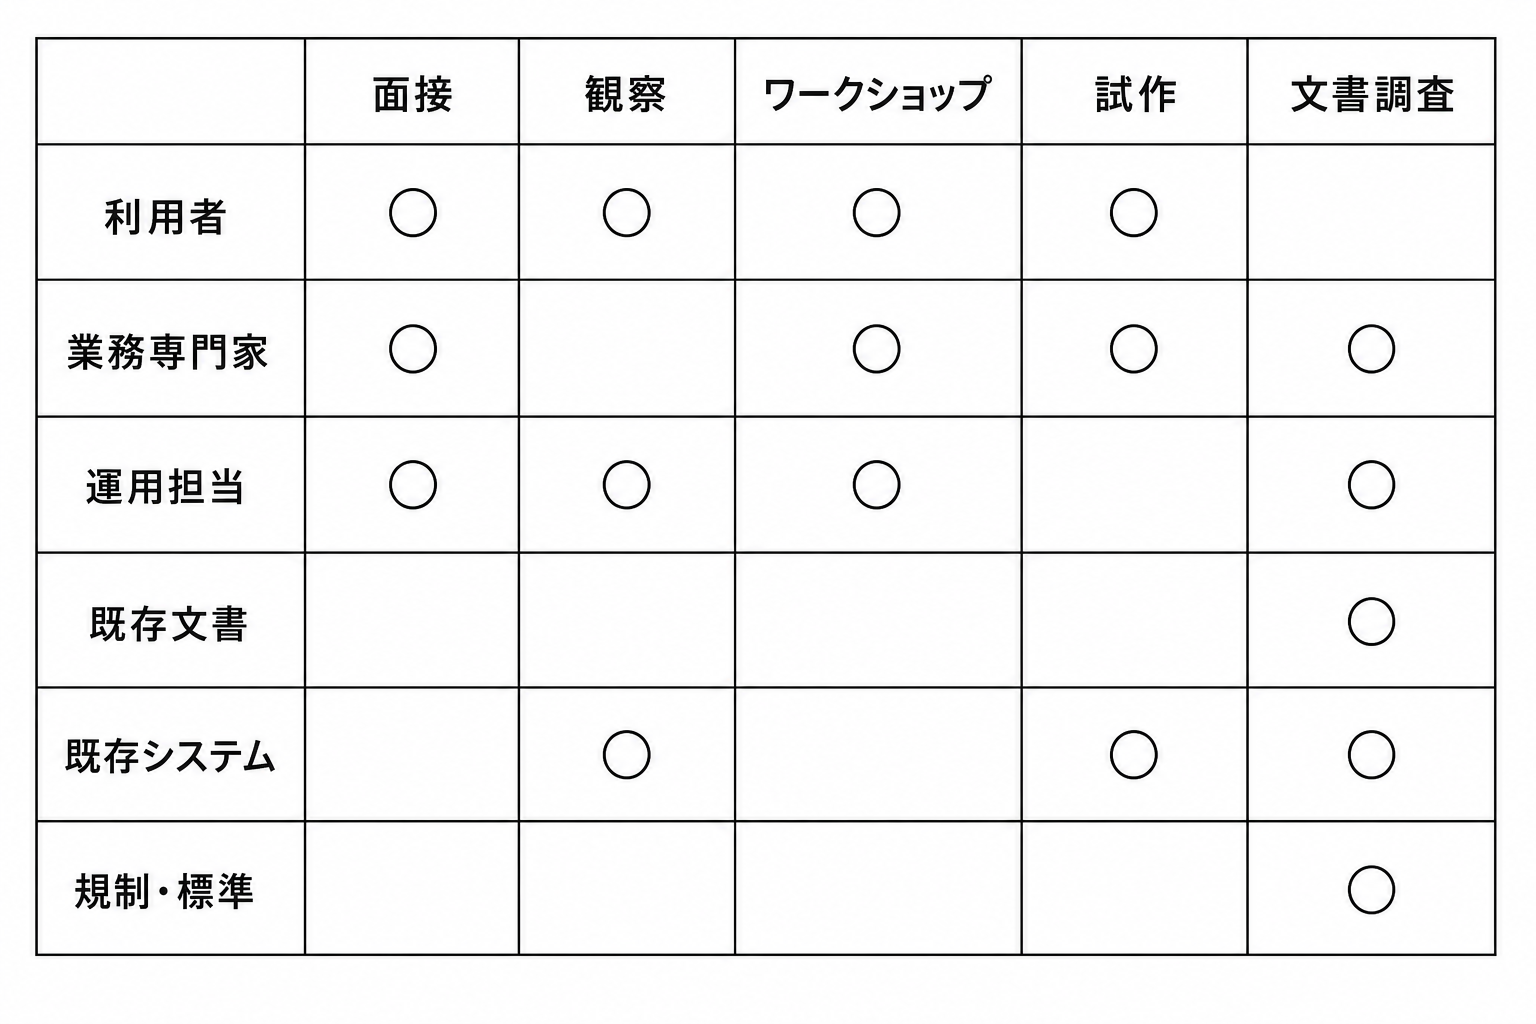
\includegraphics[width=0.96\linewidth]{swebok_structure/CH01.ソフトウェア要求(Software_Requirements)/1.2.要求獲得(Requirements_Elicitation)/1.2.2.一般的な要求獲得技法(Common_Requirements_Elicitation_Techniques)/assets/fig-ch01-06.png}}{\fbox{\parbox[c][48mm][c]{0.9\linewidth}{\centering 画像生成待ち\\要求の源泉と獲得技法の対応図}}}
\caption{要求の源泉と獲得技法の対応図}
\label{fig:ch01-06}
\end{figure}

要求獲得は受け身の活動ではない。利用者は自分の作業をうまく説明できないことがある。重要な情報を当然のこととして言わないこともある。したがって、技術者は「言われたことを書くだけ」ではなく、質問し、観察し、仮説を作り、確認する必要がある。
